\documentclass[aspectratio=43]{beamer}

\makeatletter
\def\input@path{{../../inc/}}
\makeatother

\usepackage{beamerthememnrstyle}
% Eigenes Theme laden
\usetheme{mnrstyle}
\usepackage{bible_style}
\begin{document}
\begin{frame}{Inhalt}
    \begin{enumerate}
        \item \uppercase{über die bibel}
        \item \uppercase{über gott und den Menschen}
        \item \uppercase{über die Erlösung}        
    \end{enumerate}
\end{frame}
\begin{frame}{Bibel Text}
    \begin{bibelbox}{SCHL}{1Mos}{28:15}
        Gott spricht: Siehe, ich bin mit dir,
        ich behüte dich, wohin du auch gehst.
        Denn ich verlasse dich nicht,
        bis ich vollbringe, was ich dir versprochen habe.
        \end{bibelbox}
\end{frame}
\begin{frame}{Nachkommen Noahs}
    \vspace{1.5cm}
    \begin{figure}[ht]
    
    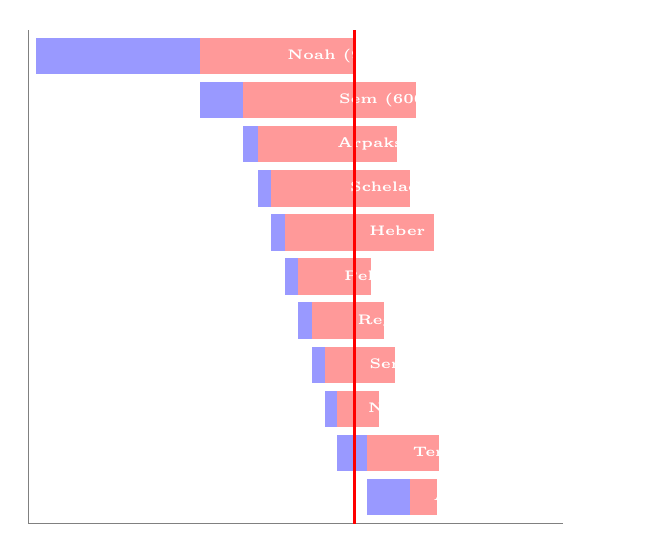
\begin{tikzpicture}[scale=.8]
    \begin{scope}[scale=0.7]
        \draw[gray] (0,0) -- (0mm, 112mm);
        
        %Noah 500-450 (0 - 93.6)
        \filldraw[blue!40] (2mm,110mm) rectangle(39mm,102mm);
        \filldraw[red!40] (39mm,110mm) rectangle(74.1mm,102mm) node[right, pos=.5, align=left, white] {\tiny \textbf{Noah (950 Jahre)}};
        
        %Sem 100-500 (0 - 93.6)
        \filldraw[blue!40] (39mm, 100mm) rectangle(48.8mm,92mm);
        \filldraw[red!40] (48.8mm,100mm) rectangle(87.8mm,92mm) node[right, pos=.5, align=left, white] {\tiny  \textbf{Sem (600 Jahre)}};
        
         %Arpakschad 35-403 (15.6 - 62.4)
         \filldraw[blue!40] (48.8mm,90mm) rectangle(52.2mm,82mm);
        \filldraw[red!40] (52.2mm,90mm) rectangle(83.6mm,82mm) node[right, pos=.5, align=left, white]  {\tiny \textbf{Arpakschad (438 Jahre)}};
        
        %Schelach 30-403 (15.6 - 62.4)
        \filldraw[blue!40] (52.2mm,80mm) rectangle(55.1mm,72mm);
        \filldraw[red!40] (55.1mm,80mm) rectangle(86.5mm,72mm) node[right, pos=.5, align=left, white] {\tiny \textbf{Schelach (433 Jahre)}};
        
        \filldraw[blue!40] (55.1mm,70mm) rectangle(58.4mm,62mm);
        \filldraw[red!40] (58.4mm,70mm) rectangle(91.9mm,62mm) node[right, pos=.5, align=left, white] {\tiny \textbf{Heber (464 Jahre)}};
        
        \filldraw[blue!40] (58.4mm,60mm) rectangle(61.3mm,52mm);
        \filldraw[red!40] (61.3mm,60mm) rectangle(77.6mm,52mm) node[right, pos=.5, align=left, white] {\tiny \textbf{Peleg (239 Jahre)}};
        
        \filldraw[blue!40] (61.3mm,50mm) rectangle(64.4mm,42mm);
        \filldraw[red!40] (64.4mm,50mm) rectangle(80.6mm,42mm) node[right, pos=.5, align=left, white] {\tiny \textbf{Regu (239 Jahre)}};
        
        \filldraw[blue!40] (64.4mm,40mm) rectangle(67.4mm,32mm);
        \filldraw[red!40] (67.4mm,40mm) rectangle(83.0mm,32mm) node[right, pos=.5, align=left, white] {\tiny \textbf{Serug (230 Jahre)}};
        
        \filldraw[blue!40] (67.4mm,30mm) rectangle(70.2mm,22mm);
        \filldraw[red!40] (70.2mm,30mm) rectangle(79.5mm,22mm) node[right, pos=.5, align=left, white] {\tiny \textbf{Nahor (148 Jahre)}};
        
        \filldraw[blue!40] (70.2mm,20mm) rectangle(77mm,12mm);
        \filldraw[red!40] (77mm,20mm) rectangle(93.0mm,12mm) node[right, pos=.5, align=left, white] {\tiny \textbf{Terach (275 Jahre)}};

        \filldraw[blue!40] (77mm,10mm) rectangle(86.8mm,2mm);
        \filldraw[red!40] (86.8mm,10mm) rectangle(92.6mm,2mm) node[right, pos=.5, align=left, white] {\tiny \textbf{Abraham (175 Jahre)}};
        \draw[gray] (0,0) -- (\textwidth, 0mm);
        \draw[red, line width=.5mm] (74mm,0) -- (74mm, 112mm);
        \end{scope}
    \end{tikzpicture}

    \caption{Lebensjahre von Noah bis Abraham}
    \label{balken_alter}

\end{figure}
\end{frame}
\end{document}